\documentclass[11pt,border=5pt]{standalone}
\usepackage{fontspec}
\setmainfont{cmunrm.otf}[BoldFont=cmunbx.otf,ItalicFont=cmunti.otf,BoldItalicFont=cmunbi.otf]
\usepackage{amsmath}
\usepackage{unicode-math}
\setmathfont{NewCMMath-Regular.otf}
\usepackage{tikz}
\usetikzlibrary{arrows.meta,patterns,angles,quotes}
\begin{document}
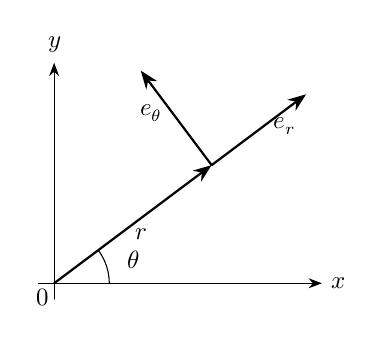
\begin{tikzpicture}[>=Stealth,font=\small,line cap=round,line join=round]
\draw[->,thin] (-0.2,0) -- (3.4,0) node[pos=1,right] {$x$};
\draw[->,thin] (0,-0.2) -- (0,2.8) node[pos=1,above] {$y$};
\node at (-0.14,-0.18) {$0$};
\draw[->,thick] (0,0) -- (2,1.5) node[pos=0.55,below] {$r$};
\draw[->,thick] (2,1.5) -- (3.2,2.4) node[pos=0.55,right] {$e_r$};
\draw[->,thick] (2,1.5) -- (1.1,2.7) node[pos=0.55,left] {$e_\theta$};
\draw (.7,0) arc (0:36.87:.7);
\node at (1,0.3) {$\theta$};

\end{tikzpicture}
\end{document}
